\documentclass{beamer}

\usepackage{listings}  % Package to include python syntax code
\usepackage{color} % Package to include colors for syntax highlighting
\usepackage{graphicx}  % Package to include images

\lstset{  % Settings for listings package
backgroundcolor=\color{cyan!10},  % Includes a light blue background color
numbers=left,  % Includes line numbers
keywordstyle=\bfseries\color{green!40!black},  % Bold and color green for keywords
identifierstyle=\color{blue},  % Other words are colored blue
stringstyle=\color{orange},  % Strings are orange
showstringspaces=false  % Don't show spaces in strings
}

\setbeamertemplate{navigation symbols}{}  % Remove navigation symbols

\title{Computing for Mathematics: Week 1}
\date{}


\begin{document}

\frame{
\titlepage
}

\frame{
\frametitle{Vince Knight}

\begin{itemize}
    \item Office: M1.25
    \item email: knightva@cf.ac.uk
    \item Office hours: Thursday 1300 - 1500
\end{itemize}

}

\frame{
\frametitle{A demo}
}

\frame{
\frametitle{Programming and Mathematics}
}

\frame{
\frametitle{Flipped classrooms}
\pause
\begin{center}
    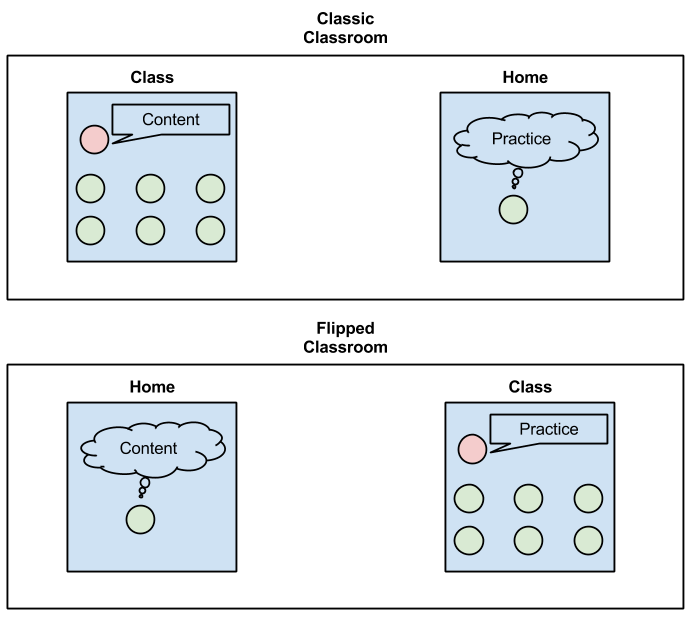
\includegraphics[width=8cm]{./images/W01-img01.png}
\end{center}
}

\frame{
\frametitle{`Tickables'}
}

\frame{
\frametitle{Resources}
}

\begin{frame}[fragile]
\frametitle{Some code}

Here is some example code:

\begin{lstlisting}[language=python]
for i in range(10):
    print 'The number is: ',i
\end{lstlisting}

\end{frame}

\end{document}
